\section{结果}

\subsection{正耦合五聚体保留低能自旋双重态}

在 $0<\alpha\leq1$ 的 100 个单胞参数点上，孤立五聚体基态始终为镜像偶宇称
$S=\frac12$ 双重态。该双重态不能在单胞内部淬灭，因而为链上的低能自由度。
最低激发双重态为奇宇称，最低四重态为偶宇称；这一宇称排序在整个正参数扫描中
保持不变。$\alpha=0$ 是额外多重态进入低能空间的边界点，因此后续有效链比较
使用严格正 $\alpha$ 的代表点。

\subsection{正胞间耦合产生反铁磁有效自旋链}

将局域自旋投影到基态双重态后，我们得到
$J_{\mathrm{eff}}/\beta=0.4396$（$\alpha=0.14$）、
$0.4318$（$\alpha=0.23$）和 $0.4189$（$\alpha=0.33$），三者均为正。
因此，正 $\beta$ 在一阶微扰中产生反铁磁自旋 $\frac12$ Heisenberg 链，而非
单胞内部完全淬灭的整数自旋链。

两五聚体完整 ED 给出的基态能量与一阶有效链之间的残差幂为
$1.9689$--$1.9915$。在 $N=8,12,16$ 的完整五聚体链 DMRG 中，相同残差幂为
$1.9483$--$1.9495$，说明首个系统修正从 $O(\beta^2)$ 开始并非两单胞偶然。
36 个最终计算 cell 全部通过能量方差、截断误差和自旋扇区门槛；四个代表点的
独立初态能量密度最大差为 $7.64\times10^{-14}$。

\subsection{有限链纠缠标度与 $c=1$ 一致}

在 $\alpha=0.23$、$\beta=0.05$ 的 $N=8$--24 开放链上，我们将五聚体链的
纠缠熵拟合与相同有效长度、相同边界和相同拟合窗口的自旋 $\frac12$
Heisenberg 链 oracle 比较。直接有限尺寸拟合仍受五站点振荡和边界修正影响，
因此不把裸拟合值解释为无偏热力学中心荷。

matched-size 校准后的估计为 $c=1.0240$--$1.0331$，相对 $c=1$ oracle 的
最大偏离为 $3.31\%$。结合正侧自旋隙在 $L=40,60,80$ 的外推接近零、
普通关联指数约为 $0.95$--$0.98$ 且静态结构因子主峰位于 $q=\pi$，这些
有限尺寸结果与反铁磁有效链的 $c=1$ 低能描述一致。它们尚不足以替代更大尺寸
和多 $\beta$ 截面的系统相图验收。

\subsection{镜像宇称过滤 $q=\pi$ 的局域激发}

最低奇宇称激发双重态在 $q=\pi$ 的谱权低于 $4.6\times10^{-27}$，尽管其
局域间隙在 $\alpha=0.14,0.23,0.33$ 分别仅为
$0.093965,0.154993,0.223495$。这一暗通道来自 $S^z(q=\pi)$ 关于单胞中心的
偶宇称，而不是有限数值精度造成的弱峰。

最低偶宇称四重态在上述三个点的间隙为
$0.143575,0.239281,0.348307$，并分别贡献约 $0.325,0.329,0.333$ 的
$q=\pi$ 谱权。整个正扫描中，所有 $S=\frac32$ 多重态合计贡献
$84.1\%$--$97.6\%$ 的局域 $q=\pi$ 非弹性权重；$S=\frac52$ 通道的
单自旋权重低于 $2.0\times10^{-28}$。

\begin{figure}[H]
  \centering
  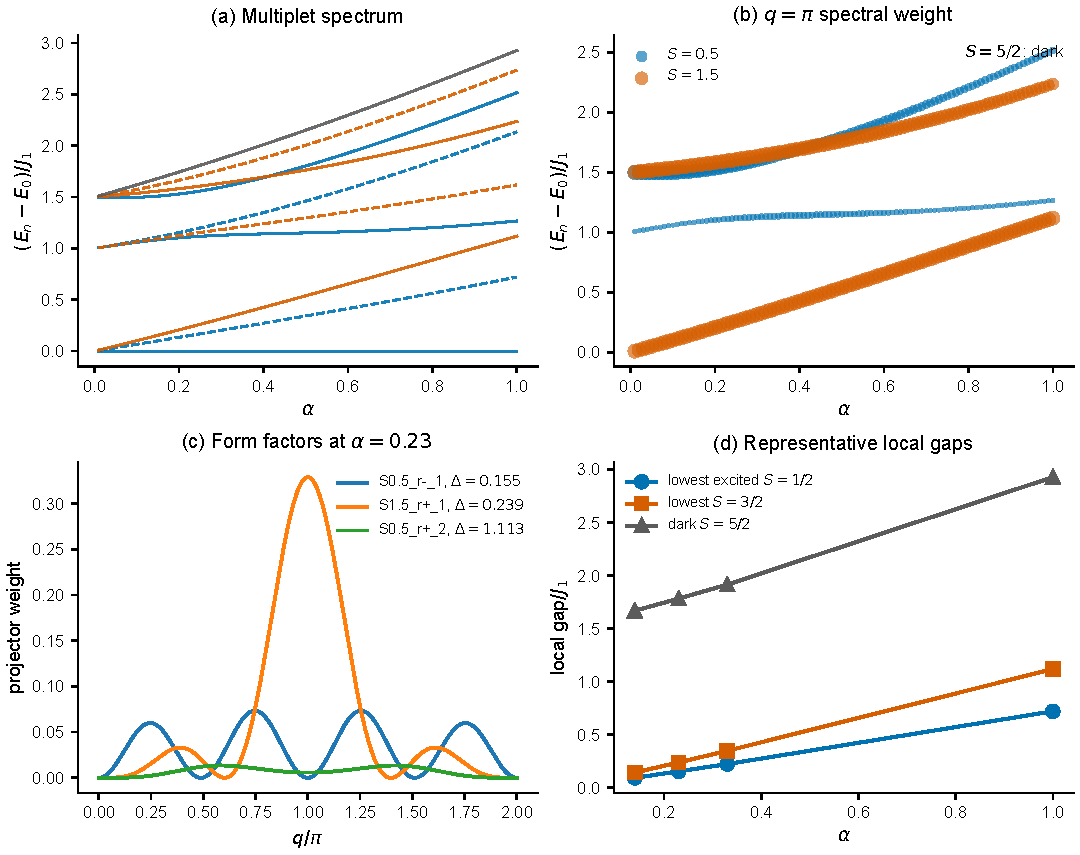
\includegraphics[width=0.98\textwidth]{positive_local_spectral_channels_20260730.pdf}
  \caption{
    通过局域谱权验收的正 $\alpha$ 五聚体激发通道。
    (a) 多重态间隙，实线和虚线分别表示镜像偶、奇宇称；
    (b) 点大小编码 $q=\pi$ 谱权；
    (c) $\alpha=0.23$ 的代表分支形状因子；
    (d) 三个正区代表点和均匀链的局域间隙。
    局域选择定则是有限 $\beta$ 动力学谱的分支先验，不等价于长链色散。
  }
  \label{fig:local-spectral-channels}
\end{figure}

\subsection{受控弱耦合区内局域四重态与两自旋子连续谱分离}

一阶有效 Heisenberg 链的热力学两自旋子连续谱具有
des Cloizeaux--Pearson 下边界
$\omega_{\mathrm L}(q)=\pi J_{\mathrm{eff}}|\sin q|/2$\cite{descloizeaux1962}，
标准两自旋子上边界为
$\omega_{\mathrm U}(q)=\pi J_{\mathrm{eff}}|\sin(q/2)|$。在 $q=\pi$
令上边界 $\pi J_{\mathrm{eff}}$ 与孤立五聚体最低四重态隙相等，可得到形式上的
嵌入阈值。对 $\alpha=0.14,0.23,0.33$，该阈值分别为
$\beta=0.10395,0.17641,0.26469$，对应
$g=\beta/\Delta_{1/2}=1.106,1.138,1.184$。

这些形式阈值均超出当前经多尺寸能隙比标定的经验受控区 $g\leq0.65$。在受控区
边缘，两自旋子上边界只达到局域四重态隙的 $54.9\%$--$58.8\%$。因此，弱耦合
有效理论预言的是低能连续谱与局域四重态之间的有限能量分离，而不是受控的嵌入或
杂化。$\beta=0.5$ 的三个动力学代表点具有 $g=2.24$--$5.32$，不能直接使用
一阶边界给强耦合谱线命名。

\begin{figure}[tb]
  \centering
  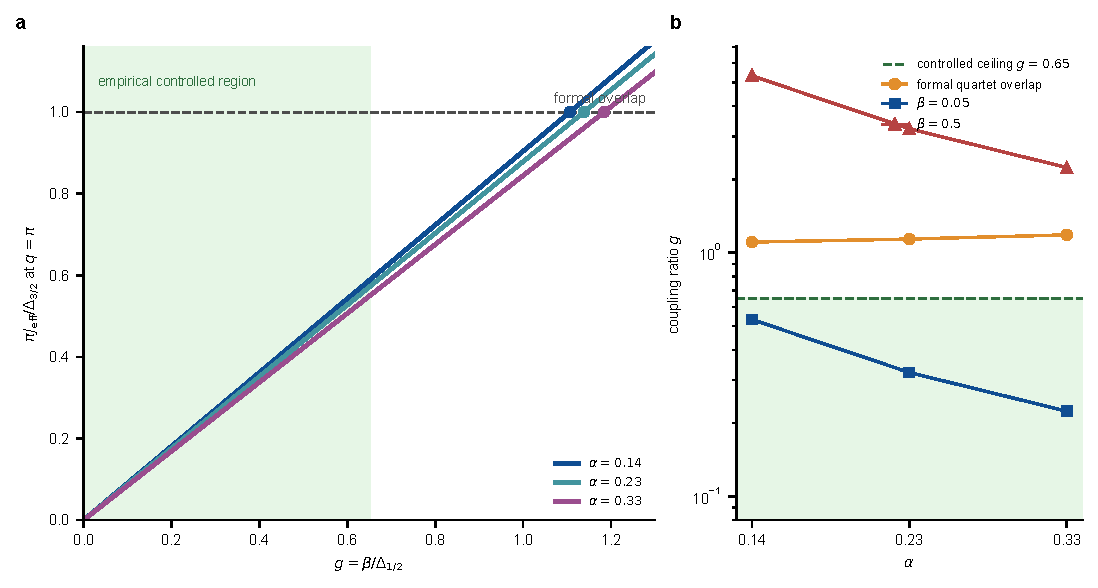
\includegraphics[width=0.98\textwidth]{effective_continuum_overlap_20260730.pdf}
  \caption{
    有效链两自旋子上边界与局域四重态的解析能量比较。
    (a) $q=\pi$ 上边界与四重态隙之比随 $g$ 的变化；绿色区域表示经有限链
    标定的经验受控区。(b) 三个代表点的受控上限、形式重叠阈值及
    $\beta=0.05,0.5$ 所在尺度。形式重叠发生在一阶投影失控后，不能解释为
    已经证明的强耦合杂化。
  }
  \label{fig:continuum-overlap}
\end{figure}

\subsection{修正向量方法通过小系统与长度标定}

在 $L=10$、总 $S^z=0$ 扇区，61 个频率点的修正向量谱与完整精确谱的相对
$L_2$ 误差为 $8.52\times10^{-12}$，积分权重相对误差为
$7.80\times10^{-13}$，最大线性方程相对残差为 $5.82\times10^{-7}$。
该结果验证了 Hamiltonian、动量源、展宽和谱归一化的一致性。

$L=20$ 单点的三档截断序列将残差从 $3.80\times10^{-4}$ 降至
$5.62\times10^{-6}$，最紧两档的谱强度相对差为 $2.33\times10^{-8}$。
$L=40$ 的相同物理点得到残差 $7.48\times10^{-6}$、实际解维数 256、
$1.50$ GiB 峰值内存和 2537 秒修正向量时间。内存不是当前瓶颈，但从
$L=20$ 到 40 的时间倍率为 16.81；在验证相邻频率 warm start 与 checkpoint
恢复前，不能据此直接提交 $L=80$ 频率网格。

\begin{figure}[tb]
  \centering
  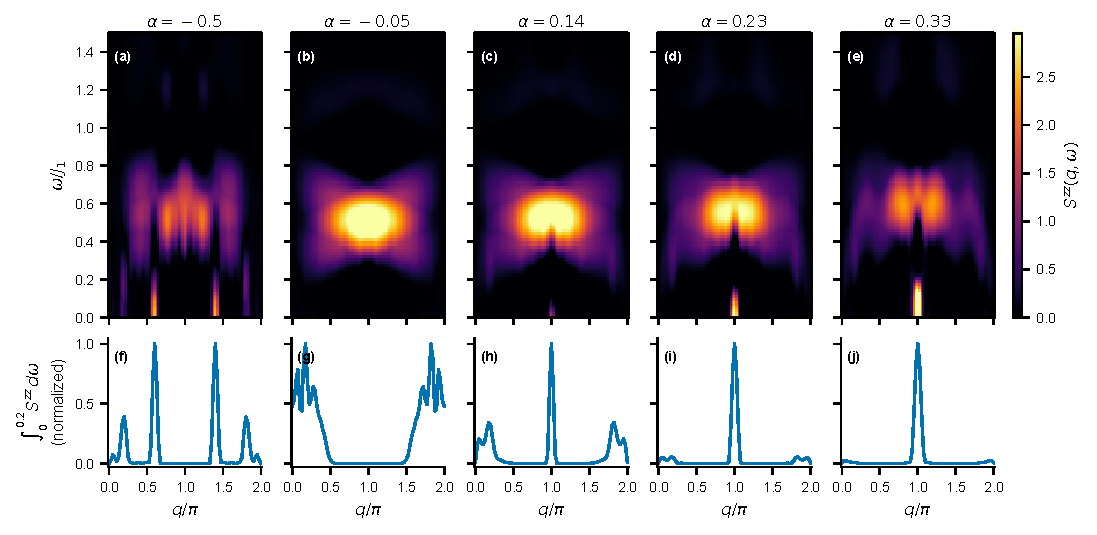
\includegraphics[width=0.88\textwidth]{Sqw_beta_half_pilot_L40_t15.pdf}
  \caption{
    $\beta=0.5$、正 $\alpha$ 代表点的试验性实时动力学结构因子。
    该图只用于定位候选低能权重；正式结论需要生产级修正向量谱、时间步长与
    最大演化时间收敛，以及两种方法的独立交叉检查。
  }
  \label{fig:pilot_dsf}
\end{figure}
